\documentclass{article}

\usepackage[utf8]{inputenc} 
% \usepackage[swedish]{babel} 
\usepackage{amsmath, amsfonts, amssymb, amsthm}
\usepackage{geometry} 
\usepackage{graphicx} 
\usepackage{hyperref} 
\usepackage{enumerate}
\usepackage{booktabs} 
\usepackage{array}
\usepackage{tikz}
\usepackage{tcolorbox}
\usepackage{pgfplots}
\pgfplotsset{compat=newest}

\geometry{a4paper, margin=1in}


\newtheorem{proposition}{Påstående}
\renewcommand{\qedsymbol}{QEB}
\tcolorboxenvironment{proposition}{
  boxrule=0pt,
  boxsep=2mm,
  colback={orange!10}, % Light orange background
  colframe={orange!50}, % Darker orange frame
  coltitle=blacf(x),
  enhanced,
  sharp corners,
  borderline west={2mm}{0pt}{orange}
}

\title{Ma5 AO5 Omfångsrika problem}
\author{Eduards Abisevs \\ Tetek-21}
\date{\today}

\begin{document}

\maketitle

\section*{Problemformulering}
I en befolkningsmodell för en stor stad kan befolkningstätheten $x$ km från
centrum approximeras med funktionen 
\[
f(x) = \frac{95\,000}{x^2 + 10x + 16}
\]
där $y$ är antalet människor per kvadratkilometer.

Uppgiften handlar om att beräkna hur många människor som bor inom en radie från
centrum.

\noindent
\subsection*{Givet}
Av uppgiften ett ledtråd. att teckna ett uttryck.

\noindent
\subsection*{Sökt}
\begin{enumerate}[(a)]
    \item Uppskatta hur många människor som bor inom en radie 5 km från centrum.
    \item Hur många människor bor mellan 5 och 10 km från centrum.
\end{enumerate}

\begin{proposition}[Befolkningsmodell inom en radie från centrum] Given nedre
	gräns \( a \) och övre gräns \( b \) där \( a,b \in \mathbb{R}^+ \)
	gäller modellen: \begin{align*}
		&\int_{a}^{b} \left(f(x) \cdot 2\pi x\right) \, dx
		= \int_{a}^{b} \frac{95\,000 \cdot 2\pi x}{x^2 + 10x + 16} \, dx
		\Rightarrow g(a,b) \\
		&g(a,b) = \frac{190\,000 \pi}{3}
		\left(4\ln{\left(\frac{b + 8}{a + 8}\right)} 
			-
		\ln{\left(\frac{b + 2}{a + 2}\right)} \right)
	\end{align*}
\end{proposition}

\begin{proof}
För att bevisa att funktionen \( g(a,b) \) gäller för godtyckliga \( a \) och \(
b \) ska integrerings processen härledas, samt resultatet av godtyckliga tal
jämföras med approxomitiv lössning med hjälp av digitala hjälp medel (Python
program).

\textbf{Steg 1} Riemannsumma
	% Circle bild
	\begin{center}
	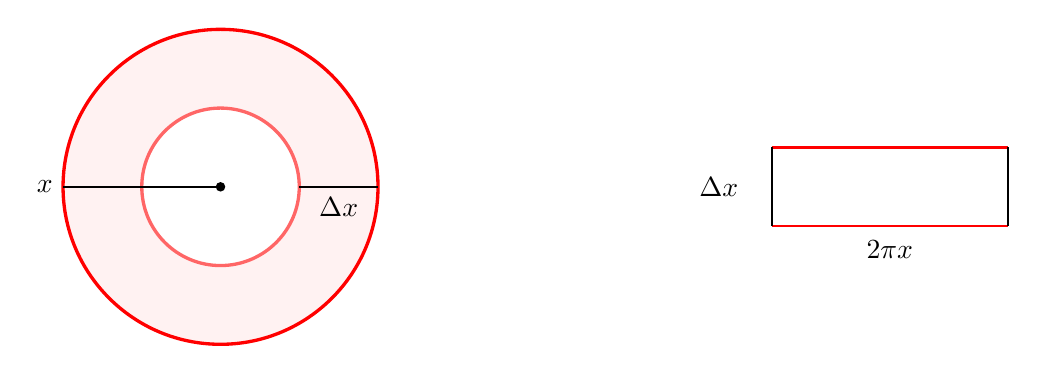
\begin{tikzpicture}
	% Define radii
	\def\rBig{2}
	\def\rSmall{1}


	% Draw the outer circle
	\filldraw[color=red, fill=red!5, very thick] (0,0) circle (\rBig);

	% Draw the inner circle
	\filldraw[color=red!60, fill=white, very thick] (0,0) circle (\rSmall);

	% Draw origo
	\filldraw[color=black] (0,0) circle (1.5pt);

	% Draw the segment indicating \Delta x
	\draw[thick] (\rSmall,0) -- (\rBig,0) node[midway, below] {$\Delta x$};
	
	% radie and annotiations
	\draw[thick] (0,0) -- (-2,0) node[left] {$x$};

	% Calculate middle point for the arrow
	\path (3,0) -- (5,0) coordinate[midway] (midpoint);

	% \draw[thick] (7,-\rSmall/2) rectangle (10,\rSmall/2);
	    % Define the coordinates for the rectangle
	\def\width{3}   % Width of the rectangle
	\def\height{1}  % Height of the rectangle
	\def\xstart{7}  % X coordinate of the starting point
	\def\ystart{-0.5} % Y coordinate of the starting point

	% Horizontal lines (black)
	\draw[thick, red] (\xstart, \ystart) -- (\xstart + \width, \ystart); % Bottom
	\draw[thick, red] (\xstart, \ystart + \height) -- (\xstart + \width, \ystart + \height); % Top

	% Vertical lines (red)
	\draw[thick] (\xstart, \ystart) -- (\xstart, \ystart + \height); % Left
	\draw[thick] (\xstart + \width, \ystart) -- (\xstart + \width, \ystart + \height); % Right
	\node at (8.5, -\rSmall/2 - 0.3) {$2\pi\/x$}; 
	\node at (7 - 0.3, 0) [left] {$\Delta x$};  
	\end{tikzpicture}
	\end{center}

	\begin{align*}
		S \approx \sum_{k=a}^{b} {f(x_k) 2 \pi \cdot \Delta x}
		% \lim_{\Delta x\to 0} \sum_{a}^{b}  \big( f(x) \cdot 2\pi x \cdot \Delta x\big) &=
		% \lim_{\Delta x\to 0} \Bigg(\frac{95\,000 \cdot 2\pi x}{x^2 + 10x + 16} \cdot \Delta x \Bigg)  \\
	\end{align*}

\textbf{Steg 2:} Låter vi $\Delta x \to 0$ övergår Reimannsumma till ett
integral
% Skriv uttrcyket för summan av små "cirkleringar" till ettintegral kalkyl
	
\begin{align*}
	g(a,b) &=\int_{a}^{b}{\left(f(x) \cdot 2\pi x\right) \, dx } \\
	       &= \int_{a}^{b}{\left(\frac{95\, 000 \cdot 2 \pi x}{x^2 + 10x + 16}\right) \, dx } \\
	&= 190\, 000 \pi \int_{a}^{b}{\left(\frac{x}{x^2 + 10x + 16}\right) \, dx }
	&&\text{(Bryta ut konstanterna)} \\
	% Visa steget hur man faktoriserer
	&= 190\, 000 \pi \int_{a}^{b}{\left(\frac{x}{(x + 8)(x + 2)}\right) \, dx }
	&&\text{(Faktorisera nämnaren)} \\
	&= 190\, 000 \pi \int_{a}^{b}{\left(\frac{A}{(x + 8)} + \frac{B}{(x + 2)}\right) \,
	dx }
	&&\text{(2.1 Simplifiera)} \\
\end{align*}

\indent
\textbf{Steg 2.1 Partialbråkupdelning}
\begin{align*}
	\frac{x}{(x + 8)(x + 2)} &= \frac{A}{x +8} + \frac{B}{x + 2} \\
				 &= \frac{A(x + 2)}{(x + 8)(x + 2)} + \frac{B(x
				 + 8)}{(x + 8)(x + 2)} \\
				 &= \frac{Ax + 2A + Bx + 8B}{(x + 8)(x + 2)} \\
				 &= \frac{x(A + B) + 2A + 8B}{(x + 8)(x + 2)}
				 \\
\end{align*}
% \indent
För att lösa ut täljaren \( A \) och \( B \) kan en enkelt ekvationssytem
defineras, där ekvationen (i) tillhör till antal \( x \)  i ursrungliga bråkets
täljare och (ii) till konstanterna.
\begin{align*}
	\begin{cases}
		A + B = 1 &(i) \\
		2A + 8B = 0 &(ii) 
	\end{cases}
\end{align*}
Ekvationen (i) omvandlas till $A = 1 - B$ och sedan sätts in i ekvationen (ii)
\begin{align*}
	&2(1 - B) + 8B = 0 \\
	&2 - 2B + 8B = 0 \\
	&6B =  -2 \\
	&B = -\frac{1}{3} \\
\end{align*}
Sätter man in B i (i) får man
\begin{align*}
	&A + (-\frac{1}{3}) = 1 \\
	&A = 1 + \frac{1}{3} \\
	&A = \frac{4}{3}
\end{align*}
Lössningen till ekvationssystemet är 
\begin{align*}
	\begin{cases}
		A = \frac{4}{3} \\
		B = - \frac{1}{3}
	\end{cases}
\end{align*}

\textbf{Steg 2.2 Lössningar till \( A \) och \( B \) sätts i integralen}
\begin{align*}
	g(a,b) &= \int_{a}^{b}{\left(f(x) \cdot 2\pi x\right) \, dx }\\
	       & \vdots \\
	&= 190\, 000 \pi \int_{a}^{b}{\left(\frac{A}{(x + 8)} + \frac{B}{(x + 2)}\right) \,
	dx }  \\
	&= 190\, 000 \pi \int_{a}^{b}{\left(\frac{\frac{4}{3}}{(x + 8)} 
		+ \frac{-\frac{1}{3}}{(x + 2)}\right) \,
	dx }  \\
	&\text{bryt ut minus tecken utanför integralen} \\
	&= 190\, 000 \pi \left(\int_{a}^{b}{\frac{\frac{4}{3}}{(x + 8)} \, dx} 
		- \int_{a}^{b}{{\frac{\frac{1}{3}}{(x + 2)} \,
	dx}\right) }  \\
\end{align*}

\textbf{Steg 2.3 beräkna första integralen}
\begin{align*}
	\int_a^b \frac{\frac{4}{3}}{x + 8} \, dx 
	&\Rightarrow \int_a^b \frac{a}{t} \, dt = \left[a\ln(|t|)\right]_a^b
	&&\text{där  \( a = \frac{4}{3} \) och \(t = x + 8 \) } \\
	&\Rightarrow \left[\frac{4}{3} \cdot \ln{(|x + 8|)}\right]_a^b 
	&&\text{(Sätt tilbaba \( a,t \))} \\
	&= \frac{4}{3} \cdot \ln{(|b + 8|)} 
	-  \frac{4}{3} \cdot \ln{(|a + 8|)}
	&& \text{(Sätt integrands gränser)} \\
	&= \frac{4}{3} \cdot \left(\ln{(|b + 8)} - \ln{(|a + 8|)} \right) 
	&&\text{Bryt ut } \frac{4}{3} \\
	&\Rightarrow \ln(a) - \ln(b) = \ln{\left(\frac{a}{b}\right)} 
	&&\text{(Logoritmiska egenskapen)} \\
	&\Rightarrow \frac{4}{3} \cdot \ln{\left(\frac{|b + 8|}{|a + 8|}\right)} 
	&&\text{(Simplifiera genom egenskapen)} \\ 
	&=  \frac{4\ln{\left(\frac{|b + 8|}{|a + 8|}\right)}}{3}
	&& \text{(Simplifiera genom multiplikation)} \\
\end{align*}
För att \( \ln(|t|) \) är definerat \( t > 0 \), används absolutbelopp
men för att \( a, b \in \mathbb{R}^+ \) kan
absolutbelopp utelämnas därmed gäller:
\[
	\int_a^b \frac{\frac{4}{3}}{x + 8} \, dx 
	= \frac{4\ln\left(\frac{b + 8}{a + 8}\right)}{3}
\]

\textbf{Steg 2.4 beräkna andra integralen} \\
Andra integralen beräknas på exakt samma sätt som första för att den är av

samma sorts.
\begin{align*}
	\int_a^b \frac{\frac{1}{3}}{x + 2} \, dx 
	&= \left[\frac{1}{3} \cdot \ln{(x + 2)}\right]_a^b  \\
	&= \frac{\ln{(b + 2)}}{3} - \frac{\ln{(a + 2)}}{3} \\
	&= \frac{\ln{(b + 2)} - \ln{(|a + 2|)}}{3} \\
	&= \frac{\ln\left({\frac{{b + 2}}{{a + 2}}}\right)}{3} \\
\end{align*}

\textbf{Steg 2.5 sätt beräknade integralerna tillbaka}
\begin{align*}
	g(a,b) &= \\
	       &\vdots \\
	       &= 190\,000\pi \left( 
\frac{4\ln{\left(\frac{b + 8}{a + 8}\right)}}{3}
- \frac{\ln\left({\frac{{b + 2}}{{a + 2}}}\right)}{3}
	       \right) \\
	       &= 190\,000\pi \left( 
		       \frac{4\ln{\left(\frac{b + 8}{a + 8}\right)}
		       - \ln\left({\frac{b + 2}{a + 2}}\right)}
		       {3} 
	       \right) 
	       &&\text{(Simplifiera under ett bråk streck)} \\
	       &= 190\,000\pi \cdot
		       \frac{1}{3}  
	       \left( 
		       4\ln{\left(\frac{b + 8}{a + 8}\right)}
		       - \ln\left({\frac{b + 2}{a + 2}}\right)
	       \right)
	       &&\text{(Faktorisera ut \( \frac{1}{3} \) )} \\
	       &= \frac{190\,000\pi}
		       {3}  
	       \left( 
		       4\ln{\left(\frac{b + 8}{a + 8}\right)}
		       - \ln\left({\frac{b + 2}{a + 2}}\right)
	       \right)
	       &&\text{(Simplifiera bråk)} \\
\end{align*}
\end{proof}

\section*{Lösning}
\subsection*{Del (a)}
Uppskatta hur många människor som bor inom en radie 5 km från centrum.
För att lösa problemet tillämpas funktion \( g(a,b) \) från Påstånde 1, där \( a
= 0 \) d.v.s. nedre gräns börjar i centrum i storstad och \( b = 5 \).  
\begin{align*}
	g(a,b) &= \frac{190\,000 \pi}{3}
		\left(4\ln{\left(\frac{b + 8}{a + 8}\right)} 
		- \ln{\left(\frac{b + 2}{a + 2}\right)} \right)
		\\ 
	g(0,5) &= \frac{190\,000\pi}{3} \left(4\ln{\left(\frac{5 + 8}{0 + 8}\right)} 
		- \ln{\left(\frac{5 + 2}{0 + 2}\right)}\right) \\
	       &= \frac{760\,000\pi \cdot \ln{\left(\frac{13}{8}\right)}}{3} 
	       - \frac{190\,000\pi \cdot \ln{\left(\frac{7}{2}\right)}}{3} 
	       &&\text{(Exakta svaret)} \\
	       &\approx 137\,142 \, \text{(Människor)}
\end{align*}

\subsection*{Del (b)}
Hur många människor bor mellan 5 och 10 km från centrum. För att beräkna detta
tillämpas funktionen \( g(a,b) \) från Påstånde 1, där \( a = 5 \) och \( b =
10 \).
\begin{align*}
	g(a,b) &= \frac{190\,000 \pi}{3}
		\left(4\ln{\left(\frac{b + 8}{a + 8}\right)} 
		- \ln{\left(\frac{b + 2}{a + 2}\right)} \right)
		\\ 
	g(5,10) &= \frac{190\,000\pi}{3} \left(4\ln{\left(\frac{10 + 8}{5 + 8}\right)} 
		- \ln{\left(\frac{10 + 2}{5 + 2}\right)}\right) \\
	       &= \frac{760\,000\pi \cdot \ln{\left(\frac{18}{13}\right)}}{3} 
	       - \frac{190\,000\pi \cdot \ln{\left(\frac{12}{7}\right)}}{3} \\
	       &\approx 151\,751 \, \text{(Människor)}
\end{align*}

\section*{Svar}
\textbf{Del (a)}: $\approx 137\,142 \, \text{(Människor)}$ \\
\textbf{Del (b)}: $\approx 151\,751 \, \text{(Människor)}$

\end{document}
